\section{Aggregation: factor analysis}

Information derived from counts of linguistic features in texts can be used in various ways for characterizing the the texts they were extracted from. In pioneering work by \cite{Biber1988,Biber1995}, factor analysis was used to identify a number of ``dimensions of variation'' that could be interpreted in terms of communicative function (such as ``narrative vs.\ non-narrative'', ``involved vs.\ informational production''), and individual texts can then be located at different points on each one of these scales. Contrasting with this multidimensional approach, there have also been attempts to automatically assign texts to a category (``genre'', ``text type'') based on the occurrence of linguistic features on those texts. A recent state-of-the-art example of such an approach is reported in \cite{EgbertBiberDavis2015}, which illustrates the enormous challenge of automatic register classification on the basis of linguistic feature counts. Using 44 linguistic features in a discriminant analysis for predicting the register category of documents from an ``unrestricted corpus of web documents'', they report precision = 0.342 and recall = 0.396 for their 20 specific sub-registers used in the task (results are generally lower when a smaller number of broader, less specific register categories is used).

In order to explore the effects of feature aggregation in predicting potentially register-sensitive morpho-syntactic alternation phenomena, we use Factor Analysis as described in \cite{Biber1988,Biber1995}. In Section~, we will treat the documents' factor scores on each one of the resulting factors as document meta, and use that meta data for modelling the outcome in specific instances of the alternation phenomenon.


\begin{figure}
   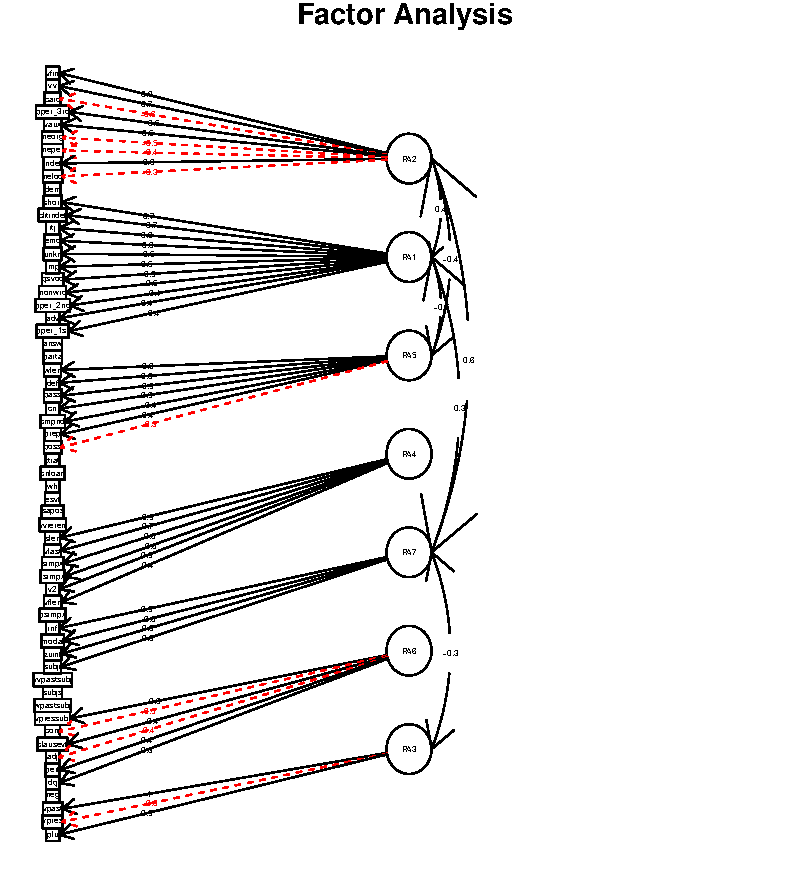
\includegraphics[scale=.9]{../R/FA-PA-7}
   \label{fa-pa-7-factors}
  \caption{Factor loadings of 60 COReX features, from a  factor analysis of 140.000 random documents (DeReKo and DECOW16 combined, minimal document length = 100 tokens), 7 factors, principal factor method, promax rotation}  
\end{figure}

